\documentclass[11pt, a4paper]{report}
\usepackage{etoolbox}
\makeatletter
\patchcmd{\chapter}{\if@openright\cleardoublepage\else\clearpage\fi}{}{}{}
\makeatother
\usepackage[margin=1in]{geometry}
\usepackage[utf8]{inputenc} % Umožňuje psaní českých znaků
\usepackage[czech]{babel}   % Česká lokalizace pro babel
\usepackage{titlesec}
\usepackage{pdfpages}
\usepackage{tabularx}
\usepackage{xcolor}
\titleformat{\chapter}
  {\normalfont\LARGE\bfseries}{\thechapter}{1em}{}
\titlespacing*{\chapter}{0pt}{3.5ex plus 1ex minus .2ex}{2.3ex plus .2ex}
\begin{document}
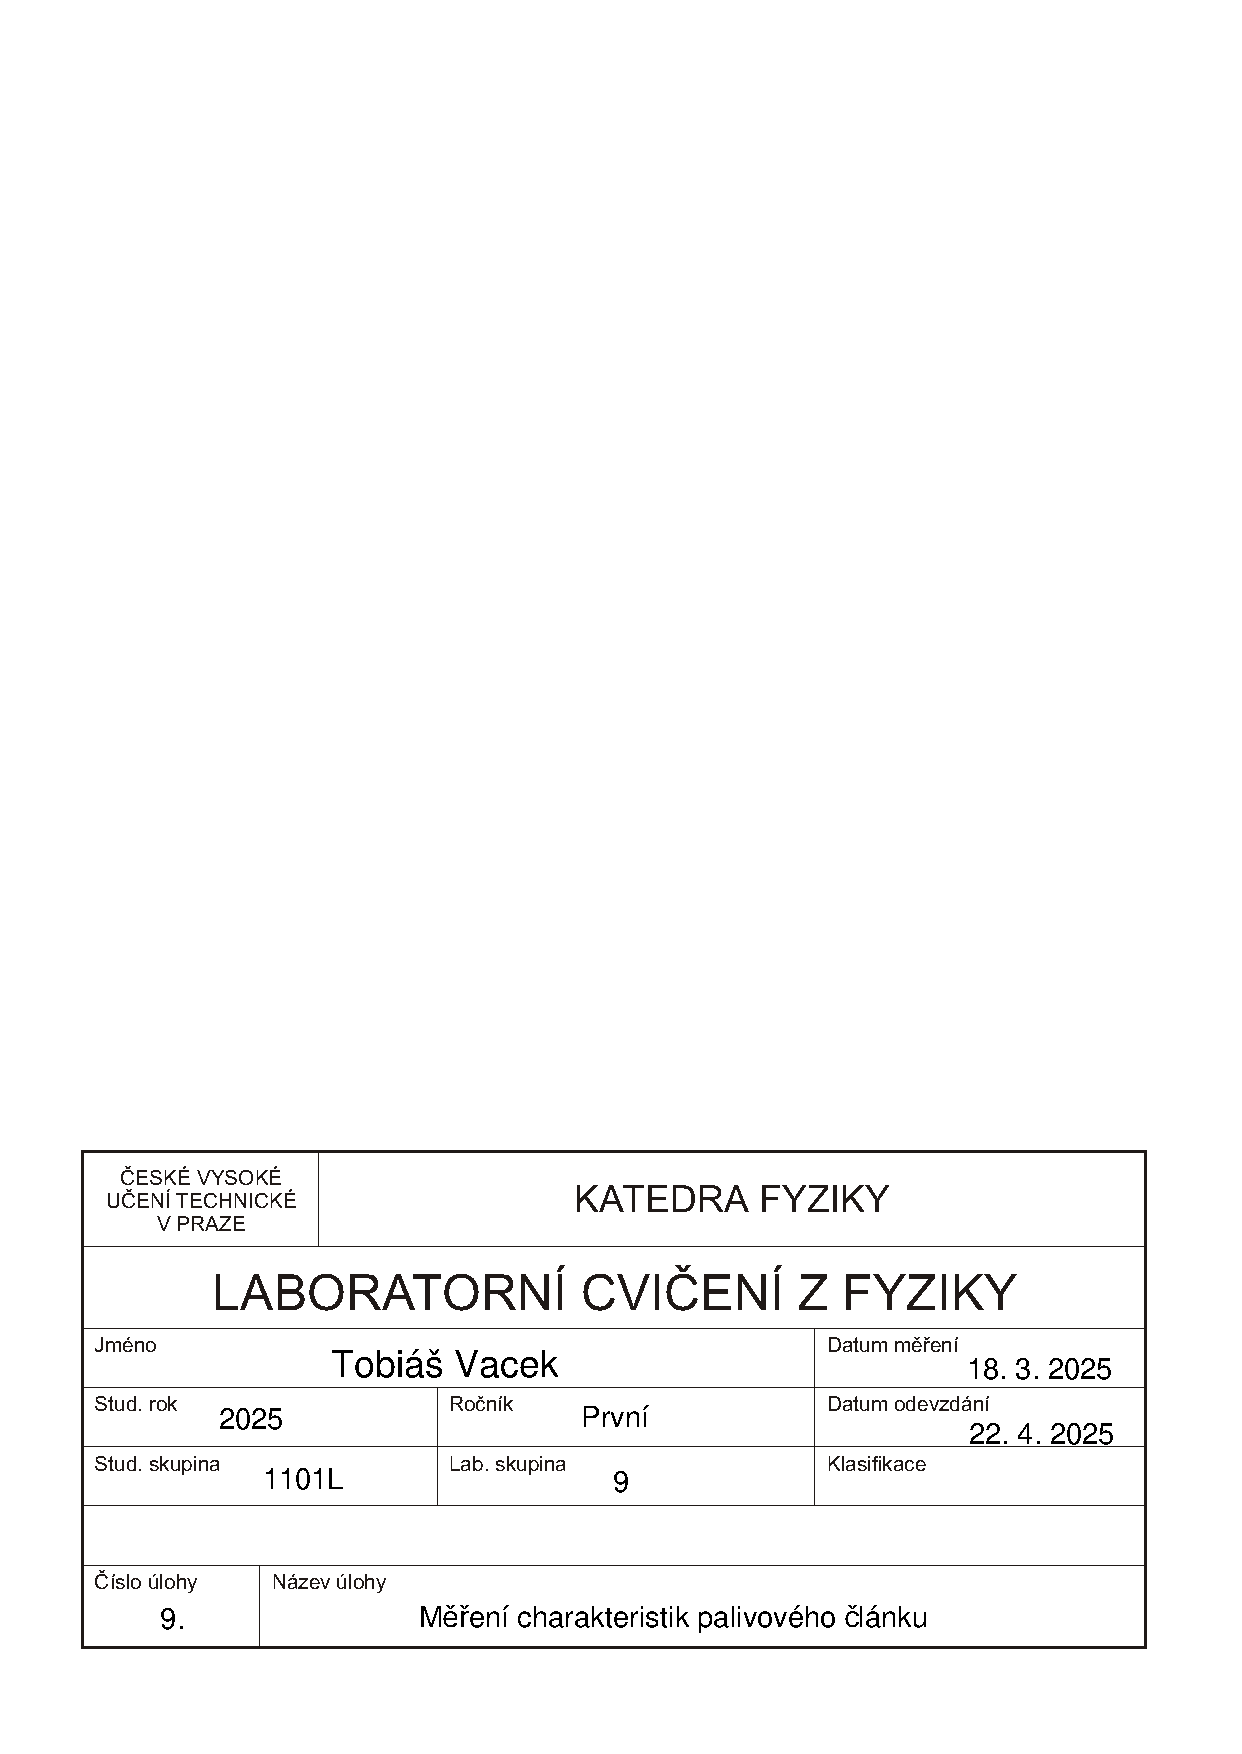
\includepdf{stamp.pdf}

\chapter{Úkol měření}
\begin{enumerate}
	\large
	\item Změřte voltampérovou charakteristiku PEM elektrolyzéru, sestrojte graf a extrapolací určete rozkladné napětí elektrolyzéru.
	\item Změřte voltampérovou charakteristiku PEM palivového článku, sestrojte graf a odhadněte maximální výkon, který lze z článku odebírat.
\end{enumerate}

\chapter{Postup měření}
\section{Příprava před měřením}
\large
Elektrolyzér byl při našem příchodu zapojen a naplněn vodou, proto jsme tyto úkony nemuseli dělat.
Začali jsme, proto kontrolou zda není palivový článek zkratován a odpojením všech zatěžovacích rezistorů.
Před zapnutím napájecího zdroje jsme nastavili výstupní napětí a omezovač proudu na nulu.
Zapnuli jsme napajecí zdroj a nastavili na něm napětí 5\,V a omezovač proudu jsme nastavili tak, aby elektrolyzérem protékal maximální proud 2\,A.
Povolili jsme všechna škrtítka na vstupu a výstupu palivového článku a minutu čekali, než se ustálí napětí na elektrolyzéru.

\section{Měření voltampérové charakteristiky elektrolyzéru}
\large
Omezovačem proudu jsme postupně snižovali proud procházející elektrolyzérem, po každé změně bylo nutné minutu počkat, než se ustálí napětí na elektrolyzéru.
Po ustálení jsme si zaznamenali hodnoty napětí a proudu z měřících přístrojů.

\section{Měření voltampérové charakteristiky palivového článku}
\large
Nastavili jsme proud elektrolyzérem opět na maximální povolenou hodnotu 2\,A.
Pro zajištění stabilních provozních podmínek jsme palivový článek na dobu pěti minut zatížili odporem 2\,$\Omega$.
Po pěti minutách jsme zátěž odpojili a změřili napětí na prázdno.
Nasledně jsme článek postupně zatěžovali různými kombinacemi odporů.
Kombinace jsme měnili sestupně.

\chapter{Seznam použitých přístrojů}


\begin{center}
	\begin{tabularx}{\textwidth}{|>{\centering\arraybackslash}X
		|>{\centering\arraybackslash}X
		|>{\centering\arraybackslash}X
		|>{\centering\arraybackslash}X
		|>{\centering\arraybackslash}X|}
		\hline
		\textbf{Počet} & \textbf{Pomůcka}    & \textbf{číslo} & \textbf{Přesnost}        & \textbf{Rozsah}                \\
		\hline
		3              & ampérmetr           & MY-65          & \pm 2\,\% (\pm 5 digitů) & 10\,A                          \\
		\hline
		2              & voltmetr            & MY-65          & \pm0,5\,\% (\pm1 digit)  & 20\,V                          \\
		\hline
		1              & voltmetr            & MY-65          & \pm0,5\,\% (\pm1 digit)  & 2\,V                           \\
		\hline
		9              & Zatěžovací rezistor & -----          &                          & 10\,Ω, 20\,Ω, 5\,Ω, 2\,Ω, 1\,Ω \\
		\hline
	\end{tabularx}
\end{center}



\chapter{Naměřené hodnoty a výpočet}
\section{Voltampérová charakteristika elektrolyzéru}
\begin{center}
	\renewcommand{\arraystretch}{1.5}
	\begin{table}[h]
		\centering
		%\renewcommand{\arraystretch}{1.5} % pro větší výšku řádků
		\begin{tabular}{|c|c|c|c|c|c|c|c|c|c|c|c|}
			\hline
			\textbf{Proud} [A]  & 2.003 & 1.816 & 1.519 & 1.300 & 1.086 & 0.888 & 0.554 & 0.460 & 0.328 & 0.176 & 0.050 \\

			\hline
			\textbf{Napětí} [V] & 3.798 & 3.404 & 3.130 & 2.941 & 2.791 & 2.650 & 2.430 & 2.375 & 2.253 & 2.102 & 1.805 \\

			\hline
		\end{tabular}
	\end{table}

	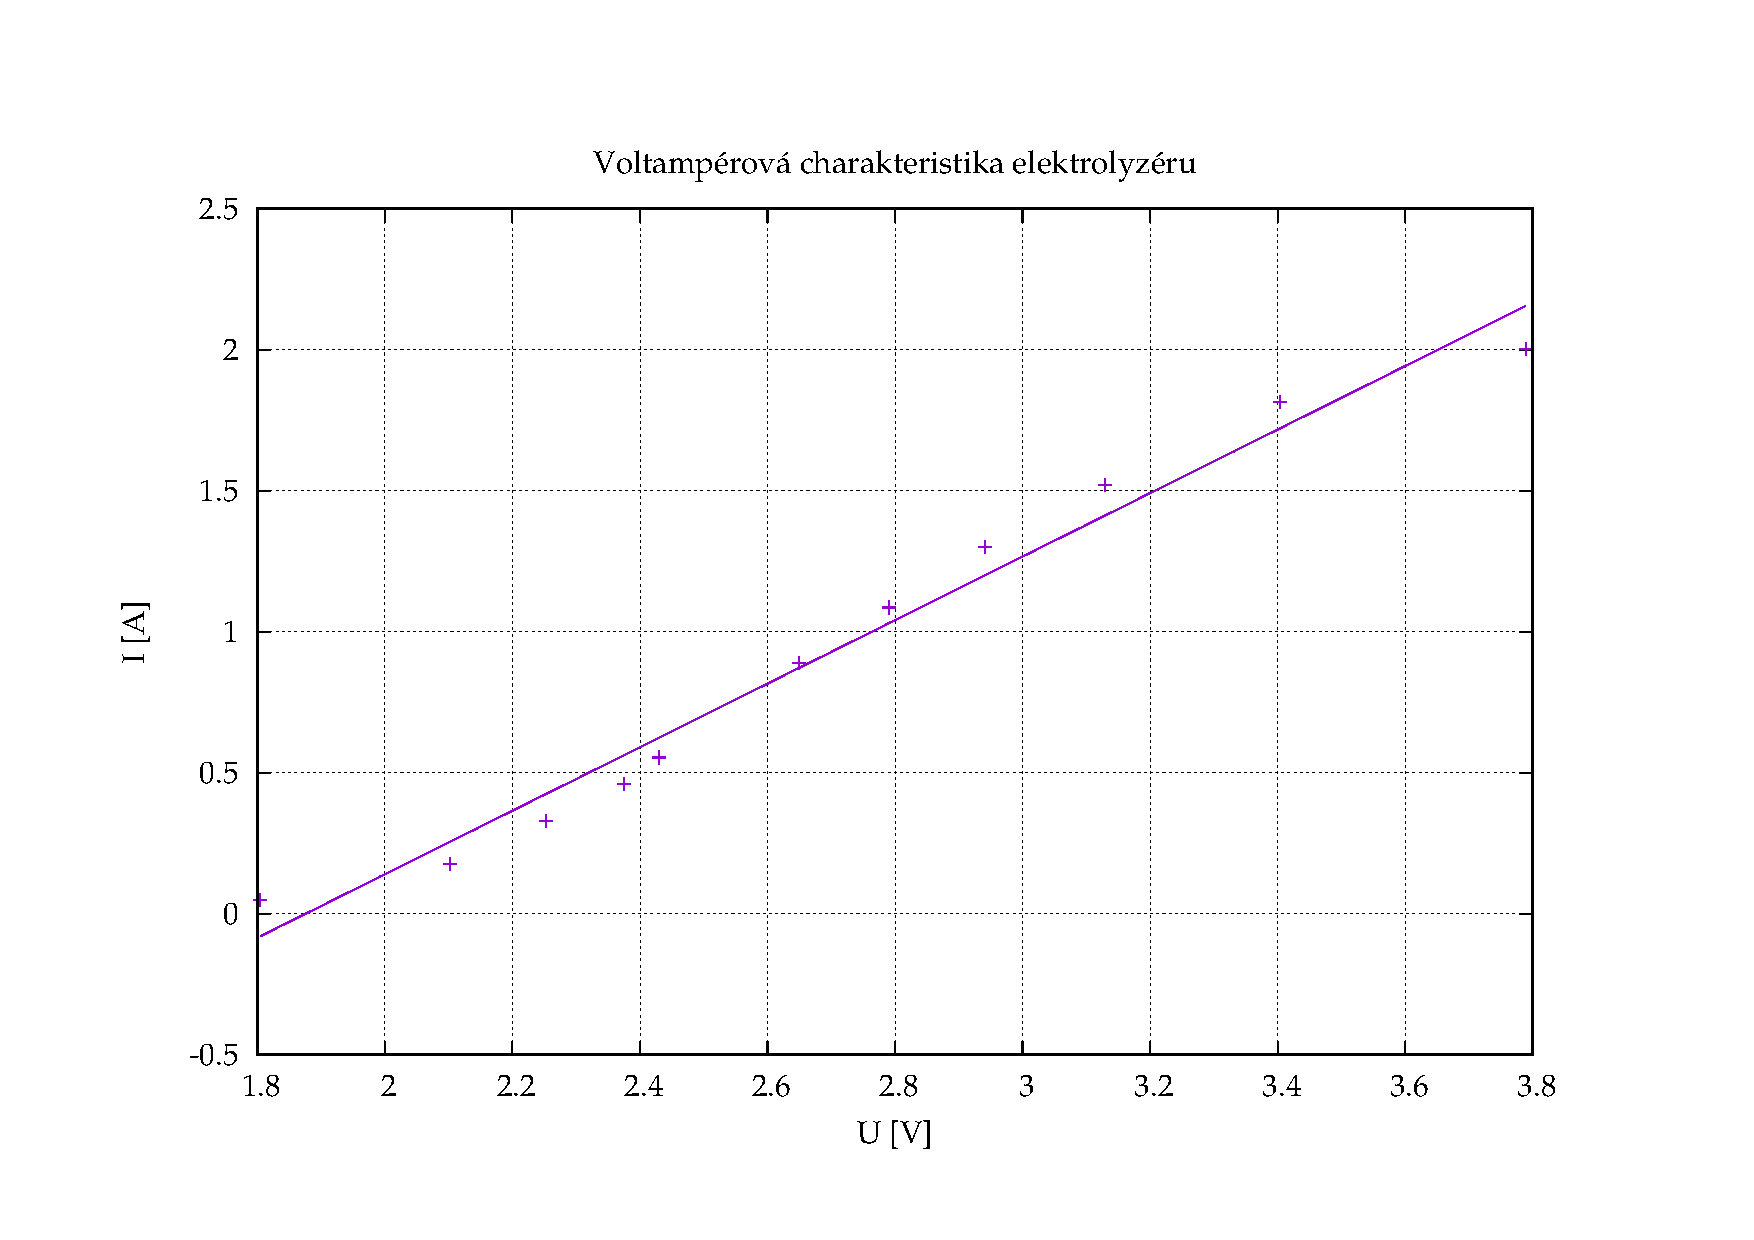
\includegraphics[width=1\textwidth, trim=2cm 1cm 3cm 1cm, clip]{VA_elektro.pdf}

\end{center}
\large
Pro určení rozkladného napětí potřebujeme závislost U(I) aproximovat přímkou ve tvaru:
\begin{center}
	\LARGE
	$I =  a_0 +a_1 \cdot U $
\end{center}
\large
Po proložení grafu přímkou na https://planck.fel.cvut.cz/praktikum/grafy/grafy.php
jsme zjistili, že hodnoty parametrů {\boldmath$a_0$ a $a_1$} jsou:

\begin{center}
	\Large
	$a_0 = -2.11 \;;\;a_1 = 1.13$
\end{center}
\large A zároveň jsme získali pomocí metody nejmenších čtverců nejistotu typu B \Large{\boldmath $u_b$ = 0.05}
\large
\clearpage
\noindent Rozkladné napětí {\boldmath$U_r$} najdeme tak, že nalezneme bod kdy přímka protíná v grafu osu X.
Položíme tedy I = 0 a dostáváme výraz:
\begin{center}
	\Large
	$0 = -2.11 + 1.13 \cdot U_r$

	$2.11 = 1.13 \cdot U_r$

	$1.89\,V \doteq U_r$
\end{center}

\section{Voltampérová charakteristika palivového článku}


\begin{center}
	\renewcommand{\arraystretch}{1.5}
	\begin{table}[h]
		\centering
		%\renewcommand{\arraystretch}{1.5} % pro větší výšku řádků
		\begin{tabular}{|c|c|c|c|c|c|c|c|c|c|c|c|}

			\hline
			\textbf{Odpor [$\Omega$]} & na prázdno & 40    & 30    & 20                 & 15    & 10    & 8     & 6     & 4     & 3     & 2     \\

			\hline
			\textbf{Proud} [A]        & 0          & 0.020 & 0.025 & 0.037              & 0.048 & 0.068 & 0.080 & 0.096 & 0.124 & 0.171 & 0.163 \\
			\hline

			\hline
			\textbf{Napětí} [V]       & 0.918      & 0.804 & 0.784 & 0.755              & 0.731 & 0.686 & 0.656 & 0.608 & 0.516 & 0.436 & 0.333 \\
			\hline
			\hline
			\hline
			\textbf{Odpor [$\Omega$]} & 1.5        & 1     & 0.5   & 0.$\overline{333}$ &       &       &       &       &       &       &       \\

			\hline
			\textbf{Proud} [A]        & 0.181      & 0.191 & 0.213 & 0.217              &       &       &       &       &       &       &       \\

			\hline
			\textbf{Napětí} [V]       & 0.270      & 0.197 & 0.111 & 0.079              &       &       &       &       &       &       &       \\
			\hline
		\end{tabular}
	\end{table}


	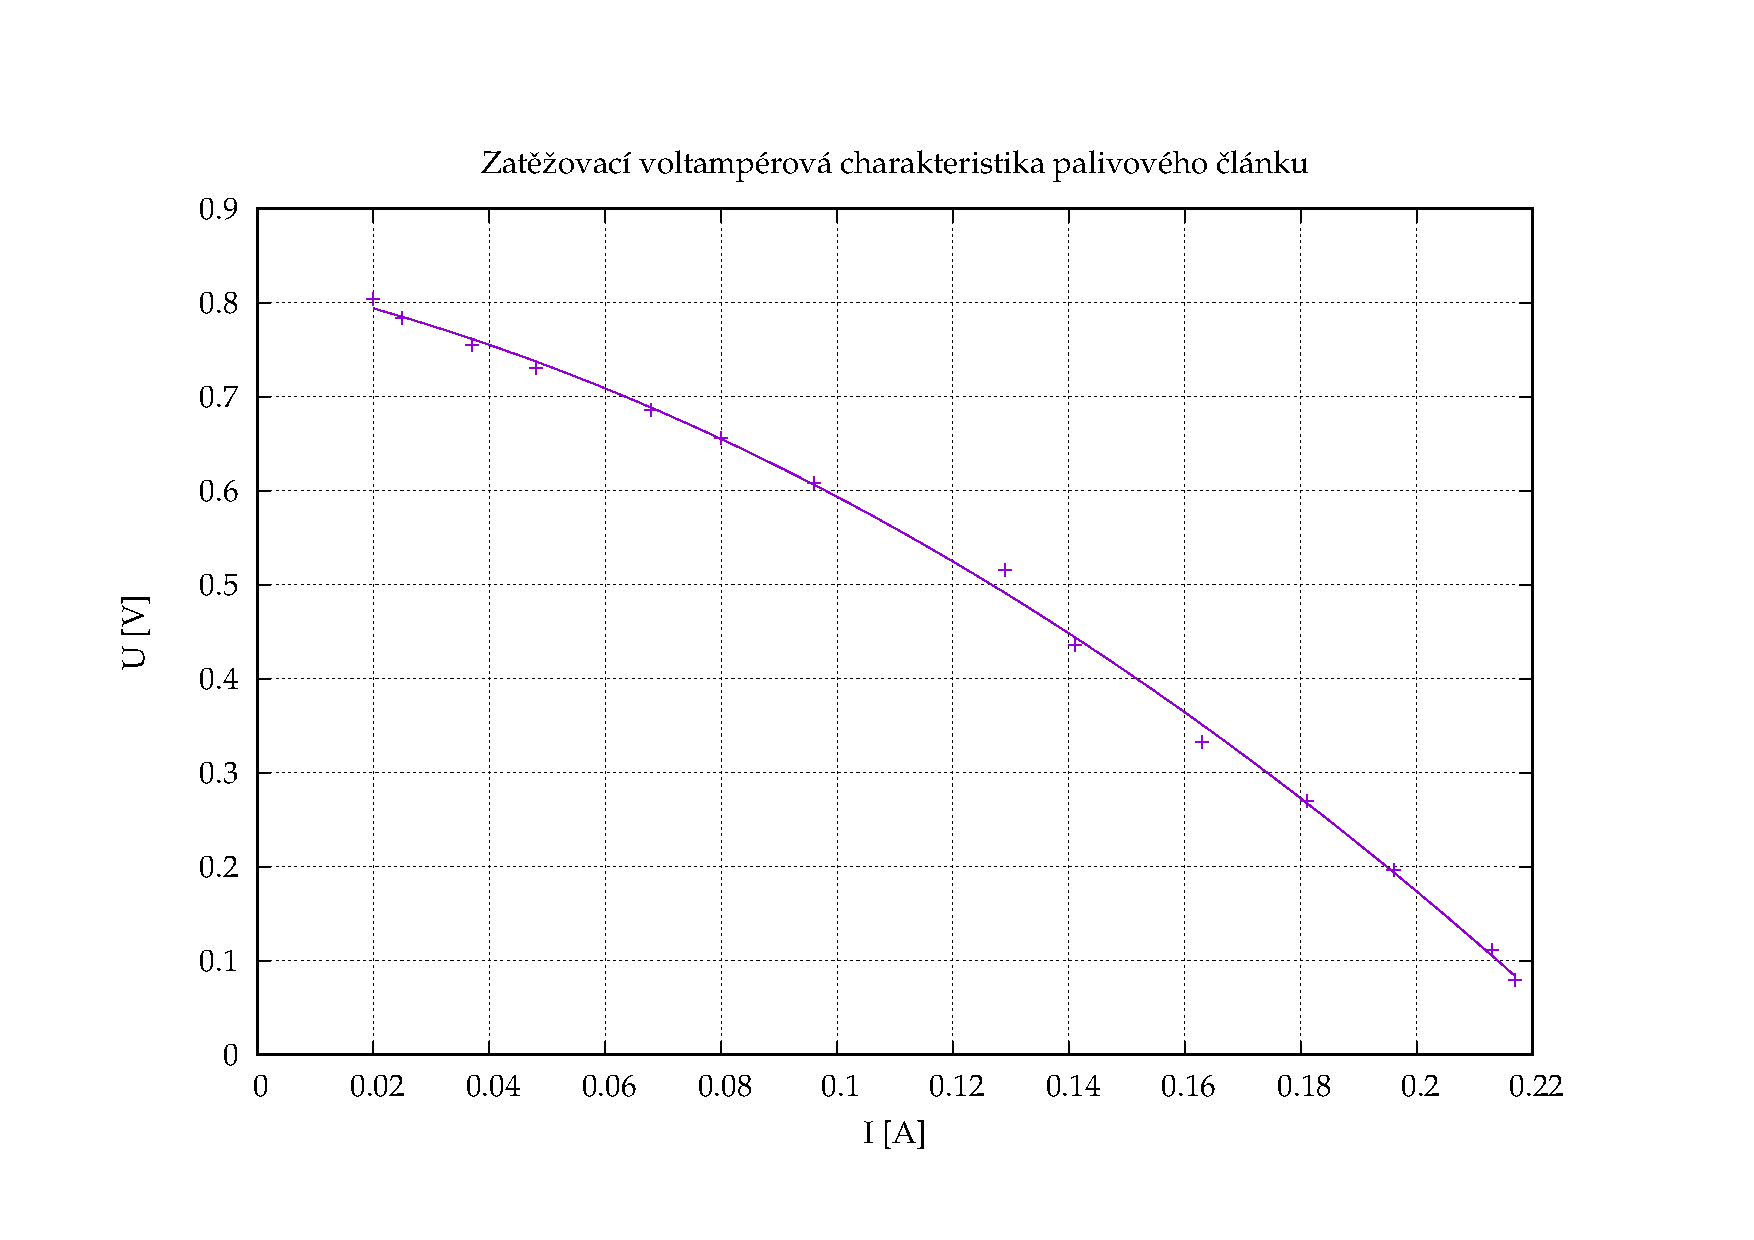
\includegraphics[width=1\textwidth, trim=1.5cm 1cm 3cm 1cm, clip]{VA_paliv.pdf}
\end{center}

\clearpage
\noindent
Výkon stejnosměrného proudu je definován jako {\boldmath $P = U \cdot I$}
Palivový článek do zátěže předá největší výkon v momentě, kdy se zátěž rovná vnitřnímu odporu článku.
Odhad maximálního výkonu, lze získat sestrojením grafu závislosti výkonu na proudu P(I) a jeho následným proložením parabolou s předpisem:
\begin{center}
	\Large
	$P = a_2 \cdot I^2 +a_1 \cdot I + a_0$
\end{center}
\large
Odhad maximálního výkonu, je pak roven vrcholu paraboly. Pro náš případ vypadají parametry {\boldmath $a_2$, $a_1$ a $a_0$} následnovně:

\begin{center}
	\Large
	$a_2 = -4.70\;;\; a_1 = 1.15\;;\; a_0 = -0.01$
\end{center}


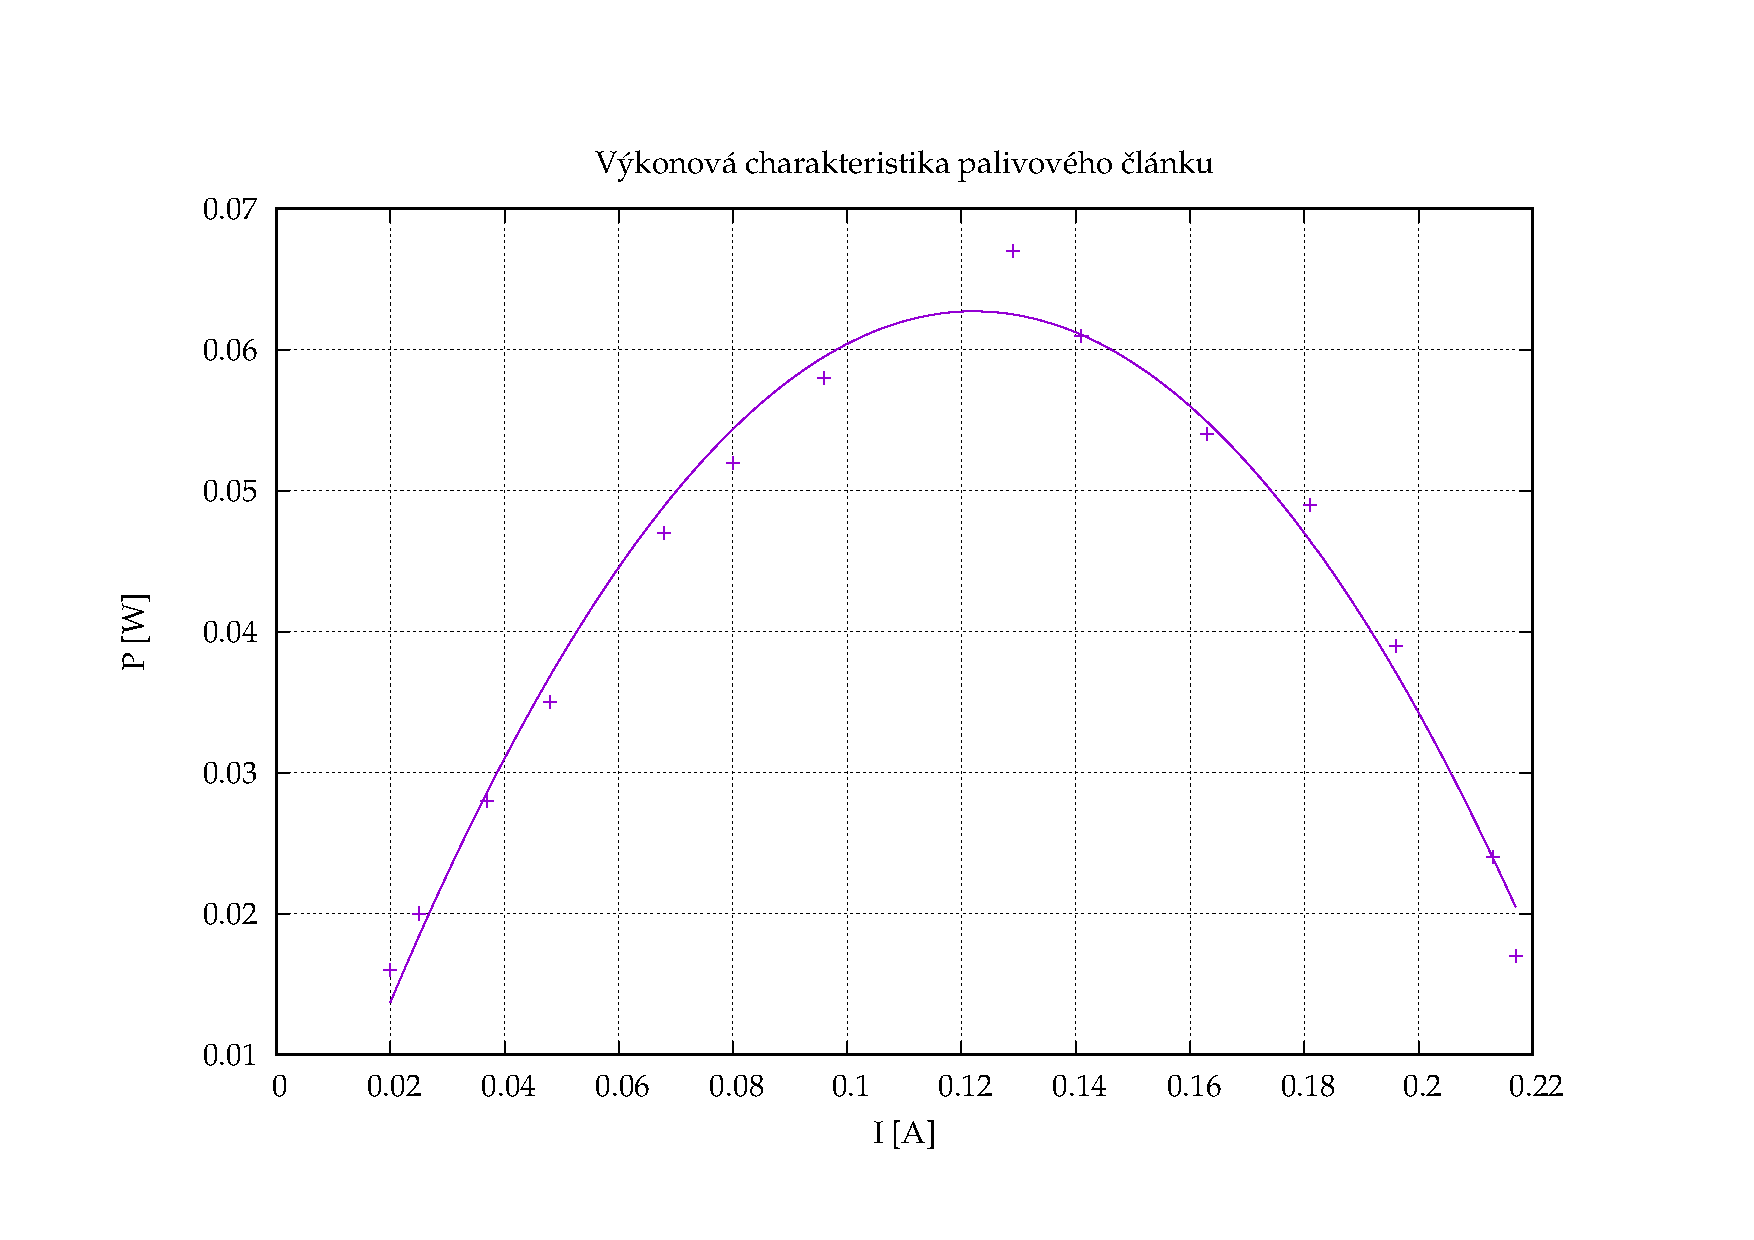
\includegraphics[width=1\textwidth, trim=1.5cm 1cm 3cm 1cm, clip]{Vykon_paliv.pdf}

\noindent Vrchol paraboly a s ním společně i náš odhad maximálního výkonu nalezneme podle vzorce:
\begin{center}
	\Large
	$vrchol = -\frac{b}{2a} => I_{max} = -\frac{a_1}{2a_2}$

	\vspace{1pt}
	$I_{max} = -\frac{1.15}{2 \cdot (-4.70)}$

	\vspace{3pt}
	$I_{max} \doteq 0.1223 $
\end{center} 
Po dosazení do $P(I_{max}) = 60.35 \cdot 10^{-3} \,W$. 
\clearpage 
\noindent Nejistotu odhadu maximálního výkonu získáme dosazením nejistot pro jednotlivé parametry do vzorce:
\begin{center}
\Large	
\[u^2_c = \sum_{i=0}^{2}(\frac{\partial P_{max}}{\partial a_i})u^2(a_i)\]
\end{center}

\noindent kde
\begin{center}
	\Large
	$P_{max} = -\frac{a_1^2}{4a_2} + a_0$
\end{center}

Vzorec pro výslednou nejistotu je tedy
\begin{center}
	\Large
	$u_c = \sqrt{(\frac{a_1^2}{4a_2^2} \cdot \sigma_2)^2 + (\frac{a_1}{2a_2} \cdot \sigma_1)^2 + (\sigma_0)^2}$

	\vspace{5pt}
	$u_c = \sqrt{(\frac{1.15^2}{4 \cdot (-4.70)^2} \cdot 0.189)^2 + (\frac{1.15}{2 \cdot (-4.70)} \cdot 0.046)^2 + (0.002)^2}$

	\vspace{5pt}
	$u_c = 0.005978$	
\end{center}
Směrodatné odchylky {\boldmath$\sigma$} jsme získali pomocí metody nejmenších čtverců na https://planck.fel.cvut.cz/praktikum/grafy/grafy.php

\chapter{Závěr}
\large 
Pomocí proložení grafu \emph{voltampérové charakteristiky elektrolyzéru} přímkou, jsme zjistili, že rozkladné napětí $U_r = (1.89 \pm 0.05)\,V$.
\newline
\noindent
Pomocí proložení grafu \emph{výkonové charakteristiky palivového článku} parabolou, jsme odhadli maximální výkon článku na $P_{max} = (0.06035\pm0.00598)W = (60.35\pm5.98)mW$. 
\end{document}